\documentclass{article}
\usepackage{graphicx}
\usepackage{float}
\usepackage{amsmath}
\usepackage{amsfonts}
\usepackage{amssymb}
\usepackage{hyperref}
\usepackage{esint}

\usepackage[a4paper, portrait, margin=0.75in]{geometry}
\setlength\parindent{0pt}

\renewcommand{\arraystretch}{1.5}

\usepackage[italian]{babel}

\hypersetup{
    colorlinks=true,
    linkcolor=black,
    filecolor=magenta,      
    urlcolor=blue,
    pdftitle={Tecnologie internet},
    pdfpagemode=FullScreen,
    }

\begin{document}
    \author{dmotrio}
    \title{Elementi di elettromanietismo}
    \date{18 Gennaio 2022}

    \maketitle
    \tableofcontents
    \listoffigures
    \listoftables

    \section{Legge di Coulomb}
\subsection{Struttura atomica}
La carica dell'elettrone è $e=1.60218 \times 10^{-19}C$(Coulomb)

\subsection{Quantizzazione della carica}
La carica del protone è $+e$, la carica dell'elettrone è $-e$ ed il neutrone ha carica 0.
La carica elettrica di un qualunque oggetto è:
\begin{equation}
    q = (N_p-N_e)\times e
\end{equation}

\subsection{Legge di Coulomb}
Interzione elettriva tra due particelle.
\begin{itemize}
    \item $a$ possiede carica $q_a$ e si trova nell'origine del sistema
    \item $b$ possiede carica $q_b$ e si trova a una distanza $r$ da $a$
\end{itemize}
La forza esercitata da $a$ su $b$ è:
\begin{equation}
    \vec{F_{ab}} = \frac{1}{4\pi \epsilon_0}\frac{q_aq_b}{r^2}\hat{r}
\end{equation}

La forza di Coulomb è la forza che agisce tra particelle cariche.


Ricorati che essedo forze hanno un verso.

\begin{itemize}
    \item $\vec{F_{ab}}$ è la forza esercitata da $a$ su $b$
    \item $\vec{F_{ba}}$ è la forza esercitata da $b$ su $a$
\end{itemize}

Questa forza è inversamente proporzionale al quadrato della distanza(se distanza x2, intensità /4).
Le particelle con la stessa carica si respingono e quelle di carica opposta si attraggono.

La forza di Coulomb è vettoriale e obbedisce alla terza legge di Newton($F_{ab} = -F_{ba}$).

La costante di proporzionalità $\frac{1}{4\pi \epsilon_0}$ vale:
\begin{itemize}
    \item $\epsilon_0 = 8.854\times 10^{-12} [\frac{C^2}{N m^2}]$
    \item $\frac{1}{4\pi \epsilon_0} = 9\times 10^{9} [\frac{Nm^2}{C^2}]$
\end{itemize}

\subsection{Principio disovrapposizione}
Se sono presenti più cariche, gli effetti delle singole forze si sommano fra di  loro essendo vettoriali.

\begin{equation}
    \vec{F} = \vec{F_1} + \vec{F_2} + \dots + \vec{F_n}
\end{equation}

\begin{equation}
    \vec{F} = \frac{1}{4\pi \epsilon_0}\Big(\frac{qq_1}{r^2_1}\hat{r_1} + \frac{qq_2}{r^2_2}\hat{r_2} + \dots + \frac{qq_n}{r^2_n}\hat{r_n}\Big)
\end{equation}
    \section{Campo elettrico}
\subsection{Campo elettrico}

\begin{figure}[h!]
    \centering
    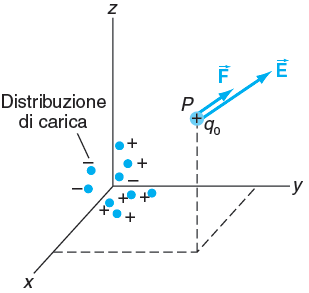
\includegraphics[width=0.3\linewidth]{imgs/1 - campo.png}
    \label{fig:campo}
    \caption{Campo elettrico}
\end{figure}

Il campo elettrico $\vec{E}$ in un punto $P$ dovuto ad un gruppo di particelle è:
\begin{equation}
    \vec{E} = \frac{\vec{F}}{q_0} [\frac{N}{C}]
\end{equation}
Dove $q_0$ è la carica di prova e la si prende piccolissima per non alterare il campo.


A volte si usa una formula più veloce avendo a che fare con tante forze singole.
Si parte dalla formula della forza:
\begin{equation}
    \vec{E} = \frac{1}{4\pi \epsilon_0}\sum{\frac{q_i}{r_i^2}\hat{r_i}}   
\end{equation}

\subsection{Distribuzione continua di cariche}
In base alla distribuzione di carica si hanno tre casi:

\subsubsection{Distribuzione di carica di volume}
$dq = \rho dv$ dove $\rho$ è la densità di carica di volume $[\frac{C}{m^3}]$.

\begin{equation}
    \vec{E} = \frac{1}{4\pi \epsilon_0}\iiint{\frac{\rho}{r^2}\hat{r}dv}
\end{equation}
\subsubsection{Distribuzione di carica di superficie}
$dq = \sigma da$ dove $\sigma$ è la densità di carica di superficie $[\frac{C}{m^2}]$.
\begin{equation}
    \vec{E} = \frac{1}{4\pi \epsilon_0}\iint{\frac{\sigma}{r^2}\hat{r}da}
\end{equation}

\subsubsection{Distribuzione di carica di linea}
$dq = \lambda dl$ dove $\lambda$ è la densità di carica di linea $[\frac{C}{m}]$.

\begin{equation}
    \vec{E} = \frac{1}{4\pi \epsilon_0}\int{\frac{\lambda}{r^2}\hat{r}dl}
\end{equation}

\subsection{Particelle cariche in campo uniforme}
La forza elettrica $\vec{F}=q\vec{E}$, è la froza risultante.
Per la \textbf{seconda legge di Newton}, si ha che $q\vec{E} = m\vec{a}$.
Quindi si ricava che:
\begin{equation}
    \vec{a} = \frac{q\vec{E}}{m}
\end{equation}

\subsubsection{Caso particolare 1}
Particella carica inizialmente in quiete in un campo elettrico uniforme.
Si muove con accelerazione costante lungo una retta parallela a $\vec{E}$.

\begin{center}
    \begin{tabular}{|c|c|c|}
        \hline 
        $a_x=\frac{qE}{m}$ & $V_x = \frac{qE}{m}t$ & $x = \frac{1}{2}\frac{qE}{m}t^2$ \\ [0.5ex]
        \hline
    \end{tabular}
\end{center}
Due casi derivati sono:
\begin{itemize}
    \item $V_x^2 = \frac{2qE}{m}x$
    \item $V_x^2 = (\frac{qE}{m})^2t^2$
\end{itemize}

\subsubsection{Caso particolare 2}
Particella carica che entra con velocità $\vec{v_0}$ in una regione sede di campo uniforme $\vec{E}$ con $\vec{v_0}$ perpendicolare a $\vec{E}$.


\begin{center}
    \begin{tabular}{|c|c|c|}
        \hline 
        $a_y=\frac{qE}{m}$ & $a_x = 0$ & $a_z = 0$ \\ [0.5ex]
        \hline
        $v_y=\frac{qE}{m}t$ & $v_x = v_0$ & $v_z = 0$ \\ [0.5ex]
        \hline
        $y=\frac{1}{2}\frac{qE}{m}t^2$ & $x = v_0 t$ & $z = 0$ \\ [0.5ex]
        \hline
    \end{tabular}
\end{center}

\begin{figure}[H]
    \centering
    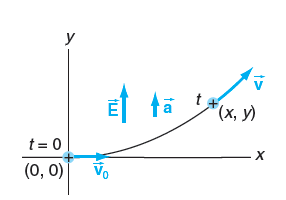
\includegraphics[width=0.3\linewidth]{imgs/2 - moto di proiettile.png}
    \label{fig:moto_parabolico}
    \caption{Moto con traiettoria parabolica}
\end{figure}
Formula del moto parabolico:
\begin{equation}
    y = \frac{1}{2}\frac{qE}{mv_0^2}x^2
\end{equation}


    \section{Legge di Gauss}

\subsection{Flusso del campo elettrico}
Il flusso $\Phi$ di un campo elettrico uniforme $\vec{E}$ attraverso una superficie piana $\Delta \vec{S}$ è:
\begin{equation}
    \Phi_E = \vec{E}\cdot \Delta\vec{S} = E\Delta S \cos\theta
\end{equation}
\begin{figure}[H]
    \centering
    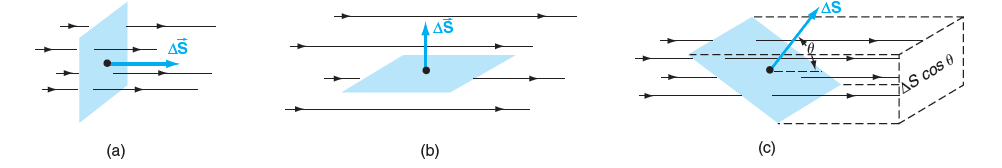
\includegraphics[width=1\linewidth]{imgs/3 - flusso gauss.png}
    \label{fig:flusso}
    \caption{Flusso rispetto al piano}
\end{figure}

\subsection{Flusso attraverso superfici non piane}
Si utilizza l'integrale.
\begin{equation}
    \Phi_E = \lim_{\Delta S_i \to 0} \sum_i{\vec{E_i}\cdot\Delta\vec{S_i}} = \iint{\vec{E}\cdot d\vec{S}} = \iint{E \cos\theta dS}
\end{equation}

Nella maggior parte dei casi si parlerà di integrali di superfici per superficie chiuse
e si indicano con il simbolo:
\begin{equation*}
    \Phi_E = \oiint{\vec{E}\cdot d\vec{S}}
\end{equation*}

\subsection{Legge di gauss}
Il flusso del campo elettrico attraverso una superficie chiusa arbitraria è pari
alla somma algebrica delle cariche contenute all'interno del volume delimitato
dalla superficie divisa per la costante dielettrica del vuoto.

\begin{equation}
    \Phi_E = \frac{Q_{int}}{\epsilon_0}
\end{equation}

\subsection{Superficie gaussiana}
La superficie chiusa attraverso la quale si calcola il flusso del campo elettrico
è solitamente una superficie geometrica immaginaria detta \textbf{superficie gaussina}.

\subsubsection{Esempio}
\begin{figure}[H]
    \centering
    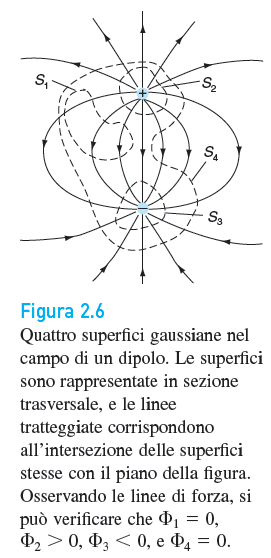
\includegraphics[width=0.25\linewidth]{imgs/4 - superficie gaussiana.png}
    \label{fig:esempio_sup_gaussiana}
    \caption{Esempio superficie gaussiana}
\end{figure}

\subsection{Campo prodotto da carica puntiforme}
\begin{figure}[H]
    \centering
    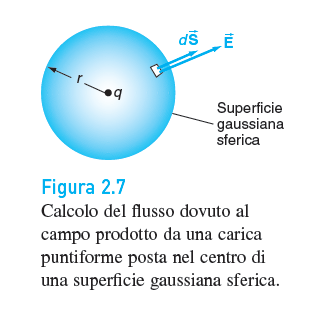
\includegraphics[width=0.25\linewidth]{imgs/5 - calcolo flusso sfera.png}
    \label{fig:esercizio_gauss_sfera}
    \caption{Campo carica puntiforme}
\end{figure}
\begin{equation}
    \Phi_E = \oiint{\vec{E}\cdot d\vec{S}} = E_r(4\pi r^2)
\end{equation}
N.B. $4\pi r^2$ è la superficie della sfera.

Se consideriamo che la carica nella sfera guassiana sia $Q_{int} = q$, 
\begin{equation*}
    \Phi_E = E_r(4\pi r^2) = \frac{q}{4\pi\epsilon_0 r^2}
\end{equation*}
Che è la stessa espressione ottenuta con Coulomb!

\subsection{legge di Coulomb $\Rightarrow$ Legge di Gauss}
\begin{figure}[H]
    \centering
    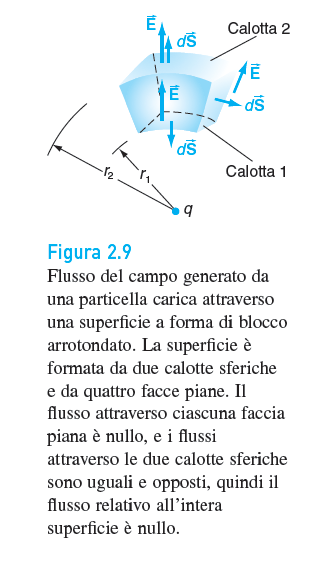
\includegraphics[width=0.25\linewidth]{imgs/6 - flusso esterno.png}
    \label{fig:carica_esterna}
    \caption{Esempio con carica esterna alla superficie}
\end{figure}

\subsubsection{Carica esterna, superficie arbitraria chiusa}
Per una qualunque superficie chiusa arbitraria ed una carica $q$ ESTERNA, il flusso vale:
\begin{equation*}
    \Phi_E = 0
\end{equation*}

\subsubsection{Carica interna, superficie arbitraria chiusa}
\begin{figure}[H]
    \centering
    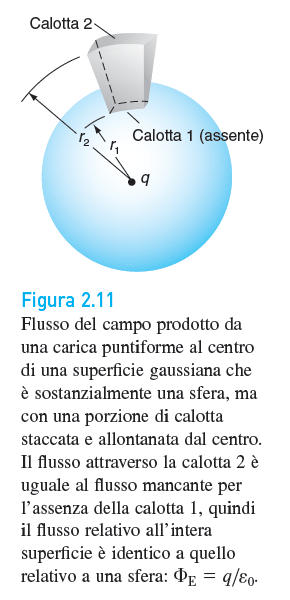
\includegraphics[width=0.25\linewidth]{imgs/7 - figura arbitraria.png}
    \label{fig:carica_interna}
    \caption{Esempio con carica interna alla superficie}
\end{figure}
Per le figure con una carica interna vale:
\begin{equation}
    \Phi_E = \frac{q}{\epsilon_0}
\end{equation}

\subsubsection{Carica sia interna che esterna con superficie chiusa}
\begin{figure}[H]
    \centering
    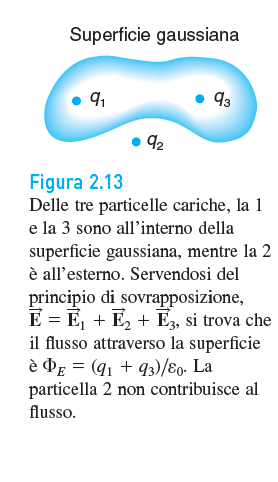
\includegraphics[width=0.25\linewidth]{imgs/8 - cariche esterne ed interne.png}
    \label{fig:carica_sia_interna_che_esterna}
    \caption{Esempio con carica esterna ed interna alla superficie}
\end{figure}

\begin{equation*}
    \Phi_E = \oiint{\vec{E}\cdot d\vec{S}} = \sum_i{\oiint{\vec{E_i}\cdot d\vec{S}}}
\end{equation*}
\begin{equation*}
    \Phi_E = \frac{Q_1}{\epsilon_0} + 0 + \frac{Q_3}{\epsilon_0}
\end{equation*}

\subsection{Legge di Coulomb Vs Legge di Gauss}
La legge di Gauss può essere dedotta da:
\begin{itemize}
    \item legge di Coulomb
    \item principio di sovrapposizione
\end{itemize}
Legge fi Coulomb può essere dedotta da:
\begin{itemize}
    \item legge fi gauss
    \item considerazioni di simmetria
\end{itemize}


\subsection{Carica con simmetria sferica}
Il campo all'esterno di una distribuzione di carica a simmetria sferica è diretto
radialmente e la sua intensità è la stessa che si avrebbe se la carica totale
fosse "concentrata" in una carica puntiforme posta al centro della
distribuzione
\begin{equation*}
    \vec{E} = \frac{q}{4\pi\epsilon_0 r^2}
\end{equation*}

\subsection{Proprietà elettrostiche dei conduttori}
\begin{itemize}
    \item Campo al'interno di un conduttore è nullo
    \item L'eccesso di carica si posiziona sulla superficie
\end{itemize}

\subsection{Campo nelle vicinanze di un conduttore}
Il campo creato dal conduttore è perpendicolare alla superficie.
In prossimità del conduttore, dove la carica di superficie $\sigma>0$, 
$E_n > 0$ avendo una intensità:
\begin{equation}
    E_n = \frac{\sigma}{\epsilon_0}
\end{equation}
    \section{Potenziale Elettrico}
\subsection{Energia potenziale elettrica}

La forza elettrica agente su un aparticella di prova è:
\begin{equation*}
    \vec{F} = q_0\vec{E}
\end{equation*}

\begin{figure}[H]
    \centering
    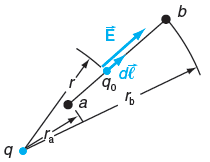
\includegraphics[width=0.2\linewidth]{imgs/9 - potenziale.png}
    \label{fig:potenziale}
    \caption{Esempio di potenziale con sfera}
\end{figure}
\begin{equation}
    \int_a^b{\vec{F}\cdot d\vec{l}} = 
    Edl\cos{90^{\circ}} = 0
\end{equation}
Dove la formula del campo elettrico è:
\begin{equation*}
    \vec{E} = \frac{q}{4\pi\epsilon_0 r^2}\hat{r}
\end{equation*}

La formula generale per calcolare il lavoro è la seguente:
\begin{equation}
    \int_a^b{\vec{F}\cdot d\vec{l}} = 
    \frac{q_0q}{4\pi\epsilon_0}
    \Bigg(\frac{1}{r_a}-\frac{1}{r_b}\Bigg)
\end{equation}

Il lavoro compiuto da una forza elettrica è indipendente dalla traiettroia.

\begin{equation}
    U_b - U_a =
    - \int_a^b{\vec{F}\cdot d\vec{l}} =
    \frac{q_0q}{4\pi\epsilon_0}
    \Bigg(\frac{1}{r_b}-\frac{1}{r_a}\Bigg)
\end{equation}
Nota che ho cambiato b con a per il segno negativo.

\subsubsection{Energia con tante cariche puntiformi}
Avendo varie cariche puntiformi, si sommano vettorialmente i loro valori.
\begin{equation*}
    \vec{F} = q_0\vec{E} = q_0\Bigg(\sum_i{\vec{E_i}}\Bigg)
\end{equation*}

\subsubsection{Formula generale}
\begin{equation}
    U = \frac{q_0}{4\pi\epsilon_0}\Bigg(\sum_i\frac{q_i}{r_i}\Bigg)
\end{equation}

\subsection{Potenziale elettrico}
\begin{equation}
    V = \frac{U}{q_0}
\end{equation}
Il potenziale prodotto in un punto P da una distribuzione di cariche:

\begin{equation}
    V = \frac{1}{4\pi\epsilon_0}\Bigg(\sum_i\frac{q_i}{r_i}\Bigg)
\end{equation}

\subsection{Elettronvolt}
\begin{equation*}
    1eV = (1.6 \times 10^{-19}C)(1V) = 1.6\times 10^{-19}J
\end{equation*}
1 eV é l'energia guadagnata da un elettrone attraverso una differenza
di potenziale di 1 V.

\subsection{Potenziale prodotto da distribuzione continua di carica}
Con il passaggio al limite, la sommatoria diventa un integrale.
\begin{equation}
    V = \frac{1}{4\pi\epsilon_0}\int\frac{dq}{r}
\end{equation}

\subsection{Differenza di potenziale}
\begin{equation}
    V_b - V_a = -\int_a^b{\vec{E}\cdot d\vec{l}}
\end{equation}

\subsection{Campo in funzione del potenziale}
\begin{equation}
    \vec{E} =
    - \Bigg(
        \frac{\delta V}{\delta x}\hat{x} +
        \frac{\delta V}{\delta y}\hat{y} +
        \frac{\delta V}{\delta z}\hat{z}
    \Bigg)
\end{equation}


\subsection{Potenziale e campo elettrico}
Potenziale e campo elettrico sono direttamente correlati:
\begin{itemize}
    \item entrambi possono essere determinati dalla distribuzione di cariche
    \item possono essere determinati a partire dall'altro
\end{itemize}

La dimensione del campo elettrico è $[\frac{V}{m}]$ o $[\frac{N}{C}]$.

\subsection{Campo elettrostatico}
Il campo elettrostatico è conservativo quando la sua cortocircuitazione è nulla.
\begin{equation*}
    \oint{\vec{E}\cdot d\vec{l}} = 0
\end{equation*}
E si può usare la fromula sia su una line ache su un volume ed una superficie,
se si usa la variazione di suerficie si usa un doppio integrale e
per il volume si usa un tripolo integrale.

\subsection{Superficie equipotenziali}
Superfici che hanno lo stesso potenziale
(come una sfera, armatura di un condensatore).

\subsection{Conduttori}
Dentro ad un conduttore, il campo E è nullo, mentre il potenziale è costante.
All'esterno entrambi decadono con l'aumetare della distanza(il campo decade più in fretta).

\begin{figure}[H]
    \centering
    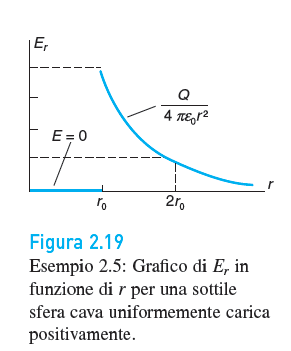
\includegraphics[width=0.25\linewidth]{imgs/10 - campo vs potenziale.png}
    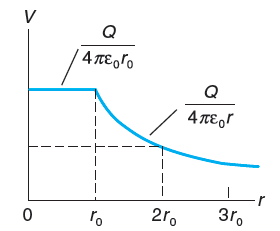
\includegraphics[width=0.25\linewidth]{imgs/11 - campo vs potenziale2.png}
    \caption{Potenziale Vs Campo}
    \label{fig:potenziale_vs_campo}
\end{figure}

\subsection{Rigidità dielettrica}
La rigidità dielettrica è il massimo campo applicabile ad un isolante prima che questo
smetta di isolare e permetta il passaggio delle cariche.
Esempio: fulmini(l'aria isola finchè il campo elettrico non è troppo grande
e tenta di scaricare verso terra).
    \include{2 - elettrostatica/5 - conduttori capacità dielettrici.tex}
    \section{Corrente e resistenza}
\subsection{Intensità di corrente elettrica}
L'intensità di corrente elettrica è la variazione di cariche in un
lasso di tempo:
\begin{equation*}
    I = \frac{dQ}{dt}
\end{equation*}

\subsection{Velocità di deriva}
Il valore assoluto della carica $dQ$, che passa nella superficie $S$
nell'intervallo $dt$:
\begin{equation*}
    dQ = nSv_ddt|q|
\end{equation*}

dove:
\begin{itemize}
    \item $n$ = densità dei portaotri di carica
    \item $v_d$ = velocità di deriva
\end{itemize}

Per ottenerer la corrente, avendo trovato la variazione di carica, 
basta dividere per il tempo.

\subsection{Densità di corrente elettrica}
La densità di corrente, partendo dalla formula di prima della corrente,
dividiamo per la sezione e otteniamo:
\begin{equation*}
    J = nv_d|q|
\end{equation*}

\subsection{Consevazione della carica elettrica}
Da questa legge si capisce che se ho una carica uscente da una superficie,
la carica all'interno della superficie, è ridotta della quantità
uscità.
Questo ragionamento viene considerato quando un conduttore cambia di dimensioni
 provocando un cambio proporzioanle di densità della carica.

 Esempio:
 \begin{equation*}
     \oiint_{Schiuso}{\vec{J}d\vec{S}} =
     \iint_{S1}{\vec{J}d\vec{S}} + 
     \iint_{S2}{\vec{J}d\vec{S}} =
     - \iint_{S1}{\vec{J}d\vec{S_1}} + 
     \iint_{S2}{\vec{J}d\vec{S_2}} 
 \end{equation*}
 Serve a rappresentare la corrente entrante e uscente come densità per sezione
 così da poter fare una proporzione per l'esercizio.


 \subsection{Resistenza e legge di Ohm}
 \begin{equation*}
     R = \frac{V}{I}
 \end{equation*}

 \subsection{Resistività}
 \begin{equation*}
     R = \frac{\rho l}{S}
 \end{equation*}

 Dove $\rho$ indica la tipologia di materiale, l indica la lunghezza e S è la superficie.

 \subsection{Legge di Ohm in funzione di densità di corrente e campo}
\begin{equation*}
    \vec{J} = \sigma \vec{E}
\end{equation*}

Un campo elettrico E produce una denstià di corrente j che dipende dalla 
conducibilità del materiale (sigma).

Riassuntone:
\begin{itemize}
    \item $\vec{J} = \sigma\vec{E}$, legge di ohm in un punto interno del materiale
    \item $V = IR$ legge di ohm in un conduttore
    \item $\rho = \frac{RS}{l}$
    \item $\sigma = \frac{l}{RS}$
\end{itemize}
Rho e sigma sono opposti.

\subsection{Semiconduttori}
Materiali che si comportano comeisolanti in certe condizioni e da conduttori
in altre condizioni.

    \section{Campo magnetico}

\subsection{Forza di Lorentz}
La forza di Lorentz descrive una particella carica $q$ con velocità
$\vec{v}$ e un campo vettoriale $\vec{B}$
\begin{equation}
    \vec{F} q\vec{v}\times\vec{B}
\end{equation}
che generano la forza magnetica.

L'andamento delle forze segue la regola della mano destra:
\begin{figure}[H]
    \centering
    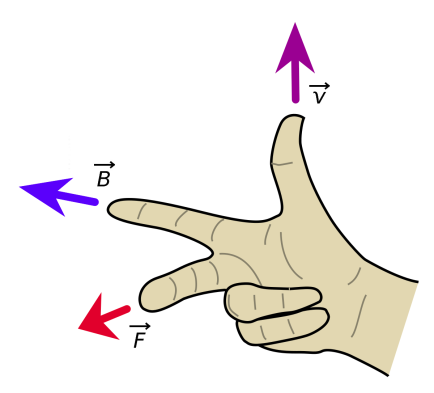
\includegraphics[width=0.2\linewidth]{imgs/12 - lorentz.png}
    \label{fig:regola_mano_destra}
    \caption{Regola mano destra}
\end{figure}

Per q positiva, la forza segue il verso di F(freccia in rosso), altrimenti ha verso opposto.

L'intensità della forza è:
\begin{equation}
    F = |qvB\sin\theta|
\end{equation}
NB:
\begin{itemize}
    \item per carica in quiete, forza = 0
    \item se v ed f solo paralleli o opposti, forza = 0
\end{itemize}

L'unità di misura è il $[T]$(Tesla), però il tesla è molto grande come unità 
di misura, perciò spesso si usa il \textbf{gauss},
$1G = 10^{-4}T$.

\subsection{Forza su un conduttore percorso da corrente}
Prima si deve ricavare il numero di portatori di carica:
\begin{equation*}
    N = nAl
\end{equation*}
dove si moltiplicano il numero dei portatoridi carica n per il volume del segmento.
La froza magnetica totale agente sulla carica $Nq$ è:
\begin{equation}
    \vec{F} = Nq\vec{v_d}\times\vec{B} = nAlq\vec{v_d}\times\vec{B}
\end{equation}

Per trovare la l'intensità della forza posso usare:
\begin{equation}
    F = IlB\sin\theta
\end{equation}

Però visto che questa frmula vale solo con fili rettilinei e campi magnetici
uniformi, bisogna integrare per ottenere il risultato nel mondo reale:
\begin{equation}
    \vec{F} = \int{Id\vec{l}\times\vec{B}}
\end{equation}

\subsection{Momento agente su una spira}
Il campo di induzione magnetica esercita una forza sul filo percorso
da corrente, può produrre un momento.

Il momento su una spira è:
\begin{equation}
    \tau = ISB\sin\theta
\end{equation}
\begin{itemize}
    \item I = corrente
    \item S = supericie
    \item B = intensità campo di induzione
    \item $\theta$ = angoolo fra vettore superficie e vettore del campo magnetico
\end{itemize}

Se invece, si ha una bobina, bisogna considerare il numero delle spire:
\begin{equation}
    \tau = NISB\sin\theta
\end{equation}
Dove N è il numero delle spire.

\subsection{Moto di cariche in presenza di campi}
La forza totale che agisce su una particella con carica q
e velocità v:
\begin{equation}
    \vec{F} = q\vec{E} + q\vec{v}\times\vec{B}
\end{equation}

Il raggio della traiettoria che assume la particella è:
\begin{equation}
    r = \frac{mv}{qB}
\end{equation}

La velocità angolare è:
\begin{equation}
    \omega = \frac{v}{r}=\frac{q}{m}B
\end{equation}
    \section{Campo magnetico}
\subsection{Legge di Biot e Savart}
Regola simile a quella del campo elettrico di Coulomb ma applicabile
al campo magnetico.
La formula è:
\begin{equation}
    d\vec{B} = \frac{\mu_0}{4\pi}\frac{Id\vec{l}\times\hat{r}}{r^2}
\end{equation}

Dove si usa la regola della mano destra pe rvedere la direzione 
e si usa la seguante formula per l'intensità:
\begin{equation}
    dB = \frac{\mu_0}{4\pi}\frac{Idl\sin\theta}{r^2}
\end{equation}

\subsection{Permeabilità magnetica del vuoto}
\begin{equation}
    \mu_0 = 4\pi \times 10^{-7} [TmA^{-1}]
\end{equation}

\subsection{Lungo filo percorso da corrente}
Si usa:
\begin{equation}
    B = \frac{\mu_0 I}{2\pi R}
\end{equation}

\subsection{Spira percorsa da corrente}
\begin{figure}[H]
    \centering
    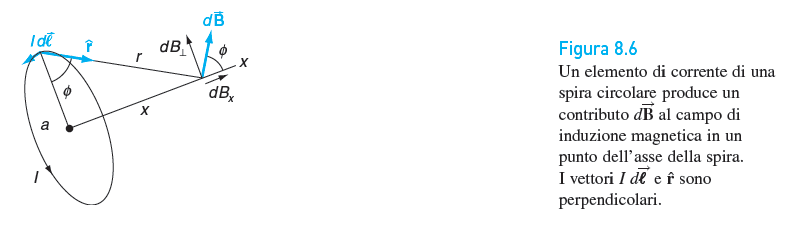
\includegraphics[width=0.5\linewidth]{imgs/13 - spira.png}
    \label{fig:spira_corrente}
    \caption{Spira percorsa da corrente}
\end{figure}
\begin{equation}
    B = \frac{\mu_IS}{2\pi(x^2+a^2)^{\frac{3}{2}}}
\end{equation}

\subsection{Legge di Ampère}
Legge usata per collegare campo magnetico e corrente concatenata.
La formula di base è:
\begin{equation*}
    B = B_1 + B_2 + ... + B_n
\end{equation*}
\begin{equation*}
    B = \sum_i{\frac{\mu_0Il_i}{2\pi R_i}}
\end{equation*}
Però spesso si cambia la lunghezza del'arco e il suo raggio con un angolo:
\begin{equation}
    B = \sum_i{\frac{\mu_0I}{2\pi}\theta_i}
\end{equation}
Questo fa capire che se l'angolo è 0, il risultato è 0(segmenti radiali non contribuiscono)

Se ho un caso dove ho più cerchi concentrici con raggi diversi, 
devo semplicemente sommare i loro contributi,
però prima devo sistemare il fatto che a raggi diverso hanno diverse intnesità.
Quindi se ho due curve, che hanno raggio1 e raggio 2,
\begin{equation*}
    B_2l_2-B_1l_1 = \frac{\mu_0I}{2\pi R_2}R_2\theta - 
    \frac{\mu_0I}{2\pi R_1}R_1\theta
\end{equation*}
Facendo così escludo i raggi dall'equazione.

\subsection{Legge della circuitazione di Ampère}
\begin{figure}[H]
    \centering
    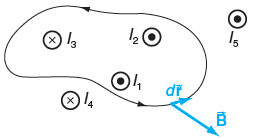
\includegraphics[width=0.3\linewidth]{imgs/14 - cortocircuitazione di ampere.png}
    \label{fig:cortocircuitazione_ampere}
    \caption{Cortocircuitazione di ampere}
\end{figure}

I4 e I5 non sono concatenate con il percorso chiuso, quindi non le considero.
Usanod la regola della mano destra attribuisco i segni alle correnti,
\begin{equation*}
    I_{conc} = I_1 + I_2 - I_3
\end{equation*}

\subsection{Legge di Ampère Vs legge di Gauss}
\begin{itemize}
    \item Ampère: campi magnetici
    \item Coulomb: campi elettrici
\end{itemize}

\subsection{Applicazione di Ampère}
Se cerco il valore esterno al lungo filo rettilineo:
\begin{equation}
    B = \frac{\mu_0I}{2\pi R}
\end{equation}

per R(distanza dal filo al punto) $>$ a(raggio del filo) e 
se il punto è sulla superficie del filo ($R=a$)

Se invece cerco il valore interno al filo:
\begin{equation}
    B = \frac{\mu_0}{2\pi R}I\frac{R^2}{a^2} = \frac{\mu_0IR}{2\pi a^2}
\end{equation}

\subsection{Campo magnetico di un solenoide}
Il solenoide ha lacaratteristica di produrre un campo tendente al nullo
all'esterno e un campo uniforme all'interno delle spire.
Maggiore è la lunghezza è il numero di spire, migliore è il risultato della 
concatenzaione.

Per trovare Il campo magnetico all'interno del solenoide, si usa La
legge di Ampère del percorso chiuso e l'unico campo non zero è quello all'interno.
Per cui vale la formula:
\begin{equation}
    B = \mu_0nI
\end{equation}
Dove $n=\frac{N}{L}$ dove rispettivamente L è la lunghezza ed N è il numero di spire.
Così facendo, si ottiene $n$ che è il numero di spire in unità di spazio.


\subsection{Forza agente tra conduttori}
Se ho due fili attraversati da corrente con segno opposto, si attraggono 
con la seguente forza:
\begin{equation}
    F = \frac{\mu_0I_1I_2}{2\pi R}l
\end{equation}
Se hanno stesso verso, si respingono con la stessa forza.
R è la distanza tra i due fili ed l è la lunghezza considerata.

\subsection{Flusso magnetico}
Come per il campo elettrico, esiste un flusso elettrico, per il campo 
magnetico esiste il flusso magnetico.
\begin{equation}
    \phi_B = \iint_S{B\cos\theta \cdot dS}
\end{equation}

L'unità di misura è il Weber(Wb), $1Wb = 1Tm^{2}$.


\subsection{Legge di Gauss per il campo elettrico}
\begin{equation*}
    \phi_E = \frac{Q_{int}}{\epsilon_0}
\end{equation*}

\subsection{Legge di Gauss per il campo magnetico}
\begin{equation*}
    \phi_B = \oiint{\vec{B}\cdot d\vec{S}}
\end{equation*}

Il flusso magnetico attraverso una superficie chiusa è nullo.


\subsection{Modifica della legge di Ampère}

\begin{figure}[H]
    \centering
    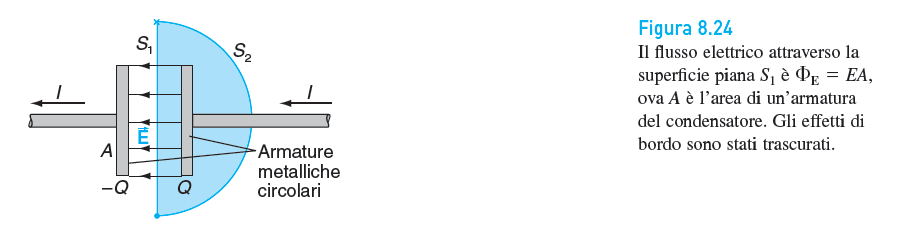
\includegraphics[width=0.8\linewidth]{imgs/16 - ampere modificata da maxwell.png}
    \label{fig:ampere_modificata}
    \caption{Ampèere modificata da Maxwell}
\end{figure}

La legge di Ampère:
\begin{equation*}
    \oint{\vec{B}\cdot d\vec{r}} = \mu_0I_{conc}
\end{equation*}
La modifica di Maxwell è:
\begin{equation}
    E = \frac{|\sigma|}{\epsilon_0} = \frac{Q}{\epsilon_0A}
\end{equation}
dove epsilon è la densità di carica dell'armatura.


\begin{equation}
    \phi_E = EA
\end{equation}
risolvendo rispetto a Q:
\begin{equation}
    Q = \epsilon_0 EA = \epsilon_0\phi_E
\end{equation}
Poi, derivando il tutto si ottiene:
\begin{equation}
    I = \frac{dQ}{dt} = \epsilon_0\frac{d\phi_E}{dt}
\end{equation}


La corrente I atraversa S2, la corrente di spostamento
IS attraversa S1 ed I=IS.

\subsection{Legge di Ampère modificata}
\begin{equation}
    \oint{\vec{B}\cdot d\vec{r}} = \mu_0\Bigg(I_{conc} + 
    \epsilon_0\frac{d\phi_E}{dt}\Bigg)
\end{equation}
    \include{3 - magnetostatica/9 - campi magnetici nella materia.tex}
    \section{Induzione elettromanietica}
\subsection{Forza elettromotrice(f.e.m.)}
La fem si misura in Volt e fornisce energia ai portaotri di cariche
per permettere il flusso di corrente.

\subsection{Induzione elettromanietica}
\begin{figure}[H]
    \centering
    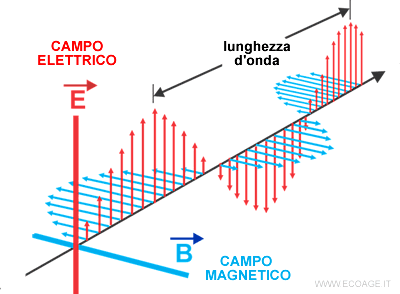
\includegraphics[width=0.3\linewidth]{imgs/17 - induzione elettromanietica.png}
    \label{fig:induzione_elettromanietica}
    \caption{Comportamento campo elettrico e magnetico}
\end{figure}
Ogni variazione del campo magnetico, provoca un campo elettrico.

\subsection{Legge di induzione elettromanietica}
La corrente indotta viene generata quando un campo magnetico varia.

\subsection{Legge di Faraday}
La fem indotta dipende dalla velocità di cariazione del flusso magnetico:
\begin{equation*}
    \epsilon = -\frac{d\phi_B}{dt}
\end{equation*}

La legge di faraday associa $1V = 1\frac{Wb}{s}$.
Se una bobina è fatta da più spire, usiamo la regola con La
concatenzaione:
\begin{equation}
    \epsilon_T = N\epsilon = N\Biggl(-\frac{d\phi_B}{dt}\Biggr)
\end{equation}

\subsection{Legge di Lenz}
Per capire il segno della fem indotta, bisogna usare Lenz.
Il senso della corrente indotta è tale che il suo contributo
al campo magnetico si oppone alla variazione del flusso magnetico
che produce la corrente indotta stessa.

Per effettuare il calcolo, bisogna definire il verso dei vettori
delta sperficie.


%TODO: Sistemare la legge di lenz perche è una merda e non volgio farla

\subsection{F.e.m. di movimento}

\begin{figure}[H]
    \centering
    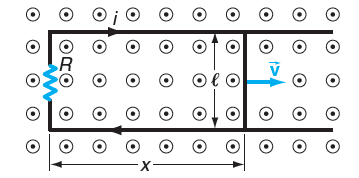
\includegraphics[width=0.4\linewidth]{imgs/18 fem indotta.png}
    \label{fig:fem_movimento}
    \caption{Fem indotta dal movimento}
\end{figure}
Il campo di induzione magnetica del circuito(perpendicolare al piano),
è:
\begin{equation}
    \phi_B = \iint{\vec{B}\cdot d\vec{S}} = Blx\cos\theta
\end{equation}

dove la $l$ e la $x$ sono l'area del circuito considerato in quel momento.

Visto che il filo scorre, l'area cambia, quindi il flusso cambia.
\begin{equation}
    \frac{d\phi_B}{dt} = \frac{d(Blx)}{dt} = Blv\cos\theta
\end{equation}
dove $v$ è la velocità(spazio fratto tempo:)).

Quindi la legge di faraday dice che la fem indotta nel circuito è:
\begin{equation}
    \epsilon = Blv\cos\theta
\end{equation}

\subsection{Campi elettrici indotti}
Se un conduttore si muove in un campo di induzione magnetica
uniforme, i portatori di carica si muoveranno con velocità
media $\vec{v}$.

La forza elettrica e magnetica agente sulle particelle è:
\begin{equation}
    \vec{F} = q(\vec{E}+\vec{v}\times\vec{B})
\end{equation}

Gli esperimenti confermano che il campo elettrico E esercita
una forza F sulla qualunque carica q presente nella regione.
La fem indotta è (più o meno) il lavoro per unità di carica
compiuto dalla forza elettrica.
\begin{equation}
    \epsilon = \frac{W}{q} = \oint{\vec{E}\cdot d\vec{l}}
\end{equation}

\subsection{Campo elettrico indotto Vs elettrostatico}
Campo elettrostatico(prodotto da una distribuzione di cariche con coulomb)
differisce dal campo elettrico indotto per:
\begin{itemize}
    \item $\oint{\vec{E}\cdot d\vec{l}} = 0$ per campo elettrostatico
    \item $\oint{\vec{E}\cdot d\vec{l}} = \epsilon$ nel campo indotto
\end{itemize}


Il campo elettrico indotto è non conservativo e viene prodotto
da un campo magnetico variabile.

\subsection{Legge di Faraday: forma integrale}
La legge di Faraday espressa in termini dei Campi è valida 
solo in presenza di conduttori, sennò cade il principio della fem.
La forma integrale(o legge generale) è:
\begin{equation}
    \oint{\vec{E}\cdot d\vec{l}} = 
    -\frac{d}{dt}\iint{\vec{B}\cdot d\vec{S}}
\end{equation}


    \section{Autoinduzione e mutua induzione}
Fino ad ora abbiamo generato una fem grazie ad un campo magnetico
esterno che interagiva con la bobina.


Adesso proviamo a fare una fem con la corrente
che gira nel filo del solenoide.

Se si usa una corrente costante, il campo (per binot e savart)
è costante.

Se si usa una corrente variabile, anche il campo sarà variabile.


Con una \textbf{condizione di correnti stazionarie}, possiamo assumere che
La fem autoindotta è:
\begin{equation*}
    \epsilon_L = -L\frac{di}{dt}
\end{equation*}

La fem autoindotta dipende dalla velocità di variazione della corrente.

\subsection{Induttanza}
$L$ è l'induttanza di una bobina, si misura in Henry$[H] = [1VsA^{-1}]$.


La fem indotta in una bobina di N spire è:
\begin{equation}
    \epsilon_L = N\frac{d\phi_B}{dt} = -L\frac{di}{dt}
\end{equation}

\subsection{Induttanza di un lungo solenoide}
Induttanza di un lungo solenoide con spire fitte:
\begin{itemize}
    \item l = lunghezza
    \item S = superficie
    \item n = numero di spire
\end{itemize}

L'intensità del campo è:
\begin{equation}
    B = \mu_0ni
\end{equation}

Il flusso concatenato è:
\begin{equation}
    \phi_B = \iint{\vec{V}\cdot d\vec{S}} = \mu_0niS
\end{equation}

In un solenoide di lunghezza l, ci sono $N=nl$ spire:
\begin{equation}
    N\phi_B = (nl)(\mu_oniS)
\end{equation}

Usando $N\phi_B = Li$, otteniamo:
\begin{equation}
    L = \mu_0n^2Sl
\end{equation}

Quindi l'induttanza dipende solo da lunghezza, sezione e 
numero di spire.


\subsection{Potenza assorbita da un'induttanza}

\begin{equation}
    P = iV = -Li\frac{di}{dt}
\end{equation}

La quantità di energia immagazzinata in una induttanza dipendente
dalla quantità di corrente:
\begin{equation}
    U = \frac{1}{2}Li^2
\end{equation}


\subsection{Energia magnetica}

Analogia tra:
\begin{itemize}
    \item energia immagazzianta in un induttore percorso da corrente($U = \frac{1}{2}Li^2$)
    \item energia immagazzinata da un condensatore($U = \frac{1}{2}\frac{Q^2}{C}$)
\end{itemize}


La densità di energia elettrica immagazzinata nel campo elettrico è:
\begin{equation}
    u_E = \frac{1}{2}\epsilon_0E^2
\end{equation}

Che è l'energia immagazzianta per unità di volume.


Stecca però per il campo magnetico è:
\begin{equation}
    u_B = \frac{B^2}{2\mu_0}
\end{equation}

\subsection{Mutua induttanza}
La fem autoindotta di una bobina influenza anche l'esterno di essa,
\begin{figure}[H]
    \centering
    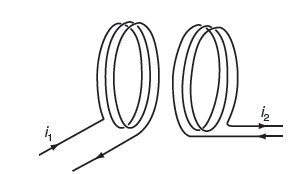
\includegraphics[width=0.5\linewidth]{imgs/19 - mutua induzione.png}
    \caption{Mutua induttanza}
    \label{fig:mutua_induttanza}
\end{figure}

La fem indotta nella bobina 1 è:
\begin{equation*}
    \epsilon_{12} = -M_{12}\frac{di_2}{dt}
\end{equation*}

Il coefficiente $M_{12}$ e $M_{21}$:
\begin{itemize}
    \item dipendono dalle proprietà geometriche del circuito
    \item vengono solitamente misurate nel circuito
    \item solo in alcuni rari casi sono facili da calcolare
\end{itemize}

La regola generale per calcolare la fem indotta in un circuito di questo tipo è:
\begin{equation}
    \epsilon_{12} = -M_{12}\frac{di_2}{dt}
\end{equation}
\begin{equation}
    \epsilon_{21} = -M_{21}\frac{di_1}{dt}
\end{equation}


\subsection{Trasformatori}
Usano la mutua induzzione per cambiare voltaggi e correnti da un circuito ad un'altro.

Solitamente si parla di primario e secondario, riferendosi al circuito 
di ingresso(primario) e al circuito di uscita(secondario).

La tensione indotta nel secondario è:
\begin{equation}
    V_s = N_s\epsilon = -N_s\frac{d\phi_B}{dt}
\end{equation}
La tensione indotta nel primario è:

\begin{equation}
    V_p = N_p\epsilon = -N_p\frac{d\phi_B}{dt}
\end{equation}

Poi spesso si utilizza semplicemente il rapporto:
\begin{equation}
    \frac{V_s}{V_p}=\frac{N_s}{N_p}
\end{equation}

E se uso le correnti, è invertito:
\begin{equation}
    \frac{I_p}{I_s}=\frac{N_s}{N_p}
\end{equation}
    \section{Equazioni di Maxwell}

\subsection{Equazioni di Maxwell}
\begin{figure}[H]
    \centering
    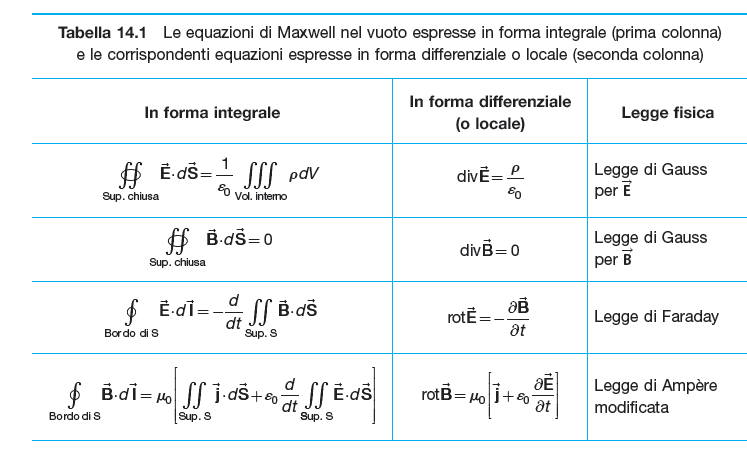
\includegraphics[width=0.8\linewidth]{imgs/20 - maxwell.png}
\end{figure}

\subsection{Legge di Gauss per il campo elettrico}

    \section{Onde}

\subsection{Caratterizzazione delle onde}
\begin{itemize}
    \item Onde meccaniche(possono esistere solo in un mezzo materiale)
    \item onde elettromeccaniche(possono esistere nel vuoto)
\end{itemize}

Per le onde meccaniche, si devono distinguere due aspetti:
\begin{itemize}
    \item moto(propagazione) dell'onda attraverso il mezzo
    \item moto della particella del mezzo materiale
\end{itemize}

\begin{figure}[H]
    \centering
    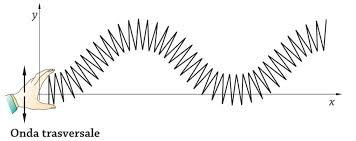
\includegraphics[width=0.45\linewidth]{imgs/22 - onda 2.png}
    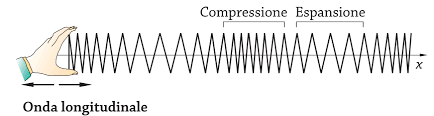
\includegraphics[width=0.45\linewidth]{imgs/21 - onde.png}
    \label{fig:onda}
    \caption{Esempio di onde in due movimenti}
\end{figure}

\subsection{Onda piana}
Una funzione d'onda è composta di $f(\vec{r},t)$ dove r è la posizione
e t il tempo.
Un'onda pina dipende solo da una direzione.



\subsection{Onde armoniche}
\begin{equation}
    f(x \pm vt) = A\sin(kx \pm \omega t + \phi)
\end{equation}

\begin{itemize}
    \item $A$ è l'ampiezza dell'onda
    \item $kx \pm \omega t + \phi$ è la fase
    \item $k$ è il numero d'onda(rad/m)
    \item $\omega$ è la pulsazione(freq angolare(rad/s))
    \item $\phi$ è la fase iniziale
\end{itemize}

Ricordati che puoi ottenere la frequenza usando $f = \frac{\omega}{2\pi}$.

L'onda armonica è progressiva/regressiva se:
\begin{equation}
    \frac{\omega}{k} = v
\end{equation}

Per l'onda progressiva, la funzione è periodica al tempo:
\begin{equation}
    T = \frac{2\pi}{\omega}
\end{equation}
e rispetto alle coordinate spaziali(lunghezza d'onda):
\begin{equation}
    \lambda = \frac{2\pi}{k}
\end{equation}

Ovviamente la velocità di propagazione sarà spazio fratto tempo:
\begin{equation}
    \frac{\lambda}{T} = \frac{\omega}{k} = v
\end{equation}

\subsection{Energia, potenza, intensità di un'onda}

La potenza si trova facendo:
\begin{equation}
    P = \frac{\Delta E}{\Delta t} = u^{(lin)}v
\end{equation}


    \section{Onde elettromanietiche}
\begin{equation}
    c = \frac{1}{\sqrt{\epsilon_0\mu_0}}
\end{equation}
Questa è una costante i cui valori sono:
\begin{itemize}
    \item $c = 2.99792458\times 10^8 [\frac{m}{s}]$
    \item $\mu_0 = 4\pi \time 10^{-7} [\frac{H}{m}]$
    \item $\epsilon_0 = 8.85 \times 10^{-12} [\frac{F}{m}]$
\end{itemize}

Con costante dielettrica relativa $\epsilon_r = \epsilon/\epsilon_0$
e permeabilità magnetica $\mu_r = \mu/\mu_0$ si ottiene:
\begin{equation}
    v = \frac{1}{\sqrt{\epsilon_0\epsilon_r\mu_0\mu_r}} = 
    \frac{1}{\sqrt{\epsilon_0\mu_0}}\frac{1}{\sqrt{\epsilon_r\mu_r}} = 
    \frac{c}{\sqrt{\epsilon_r\mu_r}}
\end{equation}

Le formule comode per la velocità sono queste:
\begin{equation}
    v = \frac{c}{\sqrt{\epsilon_r\mu_r}}
\end{equation}
Le formule comode per la rifrazione:
\begin{equation}
    n = \frac{c}{v}
\end{equation}

\subsection{Caratteristiche delle onde EM piane}

Se ho il campo magnetico o elettrico che polarizza l'onda:
\begin{equation}
    E_0 = cB_0
\end{equation}

E per le altre formule basarmi sulle formule delle onde.

\subsection{Intensità delle onde elettromanietiche}

Densità di energia associata al campo elettrico:
\begin{equation}
    u_E = \frac{1}{2}\epsilon_0E^2
\end{equation}
Densità di energia associata al campo magnetico:
\begin{equation}
    u_B = \frac{1}{2}\frac{B^2}{\mu_0}
\end{equation}

Le onde elettromanietiche piane hanno l'energia magnetica e elettrica uguale,
dato che per calcolare l'energia elettromaietica devi sommare le due,
puoi limitarti a calcolare solo una delle due:
\begin{equation}
    u_{e.m.} = u_E + u_B = 2u_B = 2u_E = \epsilon_0E^2 = 
    \frac{B^2}{\mu_0}
\end{equation}

L'intensità dell'onda è circa:
\begin{equation}
    I = A^2
\end{equation}
circa il quadrato dell'ampiezza.

Per un'onda elettromaietica:
\begin{equation}
    S = u_{e.m.}c = \epsilon_0E^2c = \frac{E^2}
    {\sqrt{\frac{\mu_0}{\epsilon_0}}}
\end{equation}
Che è l'intensità di un'onda elettromaietica.


\end{document}